% assignment_4.text - Assignment 4 for Data Fusion class (Fall 2014)
% Chanmann Lim - October 2014

\documentclass[a4paper]{article}

\usepackage[margin=1 in]{geometry}
\usepackage{amsmath}
\usepackage{listings}
\usepackage{graphicx}

\everymath{\displaystyle}

\begin{document}
\title{CS 8790: Solution to assignment 4}
\author{Chanmann Lim}
\date{October 08, 2014}
\maketitle

\subsection*{Report:} ~\\
\indent In the given data file \texttt{A3-MeasurementData.bin}, there are 100k measurements of the new 3D sensor and there exists the innovation form of the fusion equation that can be incorporated into the filter to process those data very effectively. However, several assumptions have been made for the computational advantage. Those assumptions include 1) the errors have to be independent 2) the estimates have to be unbiased with conservative covariances and 3) the estimates are in the same coordinate frame as the global coordinate frame.

\paragraph{1. } The first observation mean $z$ is just the first measurement itself and the square root of the covariance matrix R is computed with $sqrtm$ function available in Matlab.
\begin{align*}
z = \begin{bmatrix}
		12.778470 \\
		130.092667 \\
		23.529333
	\end{bmatrix}
\end{align*}
\begin{align*}
Square \; root \; of \; R = 
	\begin{bmatrix}
		0.871119    &   0.387685   &    0.301417 \\
     	0.387685    &   1.172536   &    0.689101 \\
      	0.301417    &   0.689101   &    1.560220
	\end{bmatrix}
\end{align*}

\paragraph{2. } The final mean $x$ and the new covariance $P$ are computed using innovation form of the fusion equation:
\begin{align*}
x_{new} &= x + W(z-x) \\
P_{new} &= P - WSW^{T}
\end{align*}
where
\begin{align*}
S = R + P \\
W = PS^{-1}
\end{align*}
\begin{align*}
x_{final} = 
	\begin{bmatrix}
		12.895992   \\  130.398454   \\   23.494780
	\end{bmatrix}
\end{align*}
\begin{align*}
Square \; root \; of \; P_{final} = 
	\begin{bmatrix}
        0.002755   &    0.001226   &    0.000953 \\
      	0.001226   &    0.003708   &    0.002179 \\
      	0.000953   &    0.002179   &    0.004934
	\end{bmatrix}
\end{align*}

\paragraph{3. } Plots: only the first 100 observations get plotted for visualization purpose.\\
\\
Innovation in x coordinate (blue) vs. +/- square roots of their covariances.\\
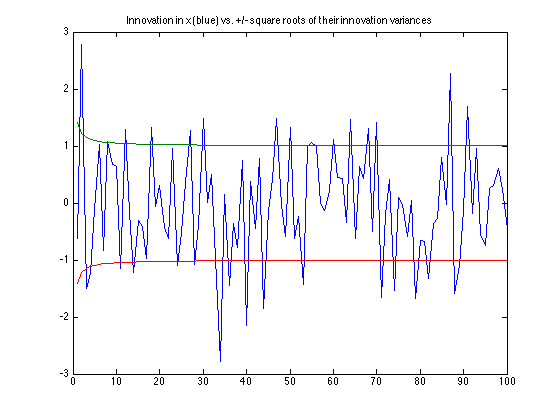
\includegraphics[scale=.8]{innovation_in_x.png}\\
Innovation in y coordinate (blue) vs. +/- square roots of their covariances.\\
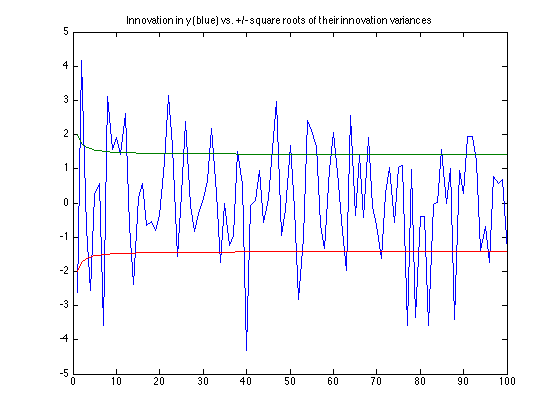
\includegraphics[scale=.8]{innovation_in_y.png}\\
Innovation in z coordinate (blue) vs. +/- square roots of their covariances.\\
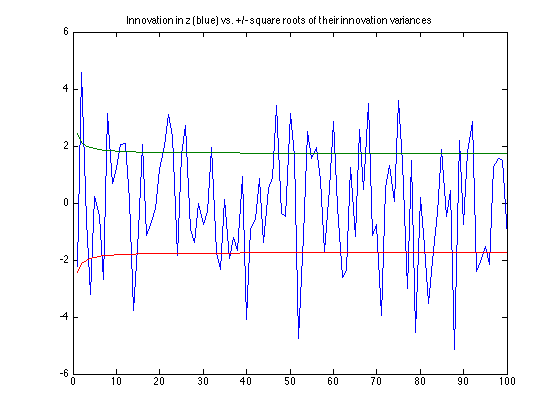
\includegraphics[scale=.75]{innovation_in_z.png}

\paragraph{4. } Plot of the estimated distance (Euclidean distance) of the mean $x$ and the ground truth $x_{True}$ (blue) vs. the expected distance (Square root of the sum of the eigenvalues of the covariance $P$) (green).\\
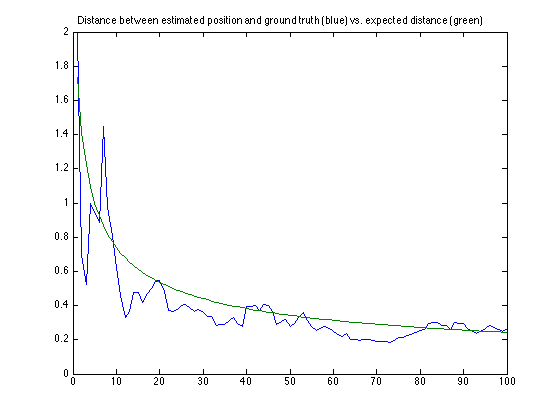
\includegraphics[scale=.75]{estimated_position.png}

\newpage
\subsection*{Appendix:}
\lstinputlisting[language=Matlab, title=\lstname, basicstyle=\footnotesize]{assignment_4.m}

\end{document}